Calcular la longitud del arco de circunferencia de radio $3$ que forma un ángulo de $60^\circ$ con el eje $x$ positivo. Comprobar la respuesta usando la fórmula para cálculo del arco de circunferencia conociendo ángulo y radio.

\nopagebreak
\begin{align*}
\text{Fórmula de longitud de arco de circunferencia: } L = r \theta. \\
r = 3, \quad \theta = 60^\circ = \pi/3. \\
L = 3 (\pi/3) = \pi. \\
\text{Por integral: } x=3\cos t, y=3\sin t. \\
L = \int_{0}^{\pi/3} \sqrt{(-3\sin t)^2 + (3\cos t)^2} \, dt \\
= \int_{0}^{\pi/3} 3 \, dt = 3(\pi/3) = \pi
\end{align*}

\[
\boxed{\displaystyle \pi}
\]

\begin{center}
    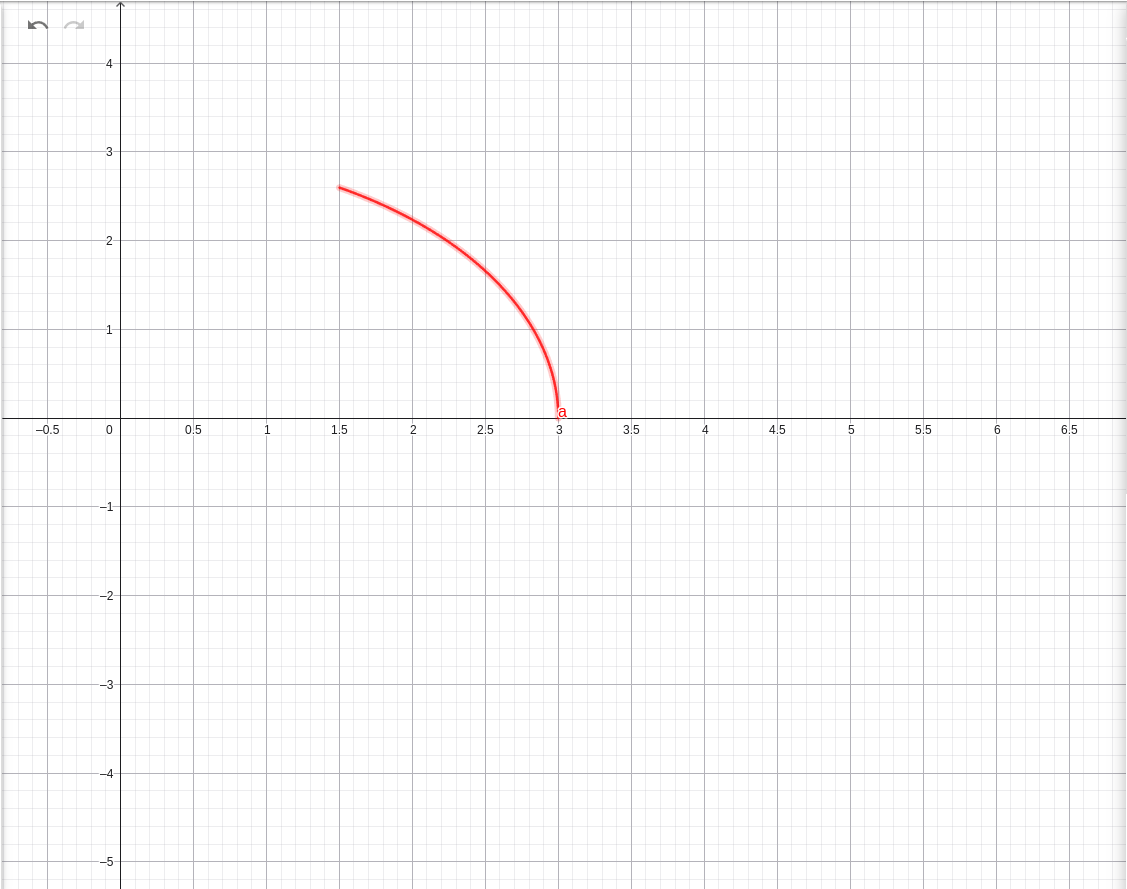
\includegraphics[width=0.5\textwidth]{Graficas/ejer50.png}
\end{center}
